Task Manager\index{task Manager} (Taakbeheer\index{taakbeheer}) is een applicatie om te zien welke applicaties er draaien, maar ook om het systeem te monitoren op CPU-belasting, geheugen-, disk- en netwerkgebruik.

Via Task Manager kan je configureren welke applicaties er opgestart worden, je kan niet reagerende applicaties afsluiten, je kan gebruikerssessies beheren en je kan services die draaien starten en stoppen.

Om Task Manager te openen:
\begin{itemize}
\item Klik op het zoek icoon en zoek op Task Manager
\item Run taskmgr.exe
\item Gebruik ctrl+shift+esc
\end{itemize}

\begin{minipage}[t]{\linewidth}
\raggedright
\adjustbox{valign=t}{%
	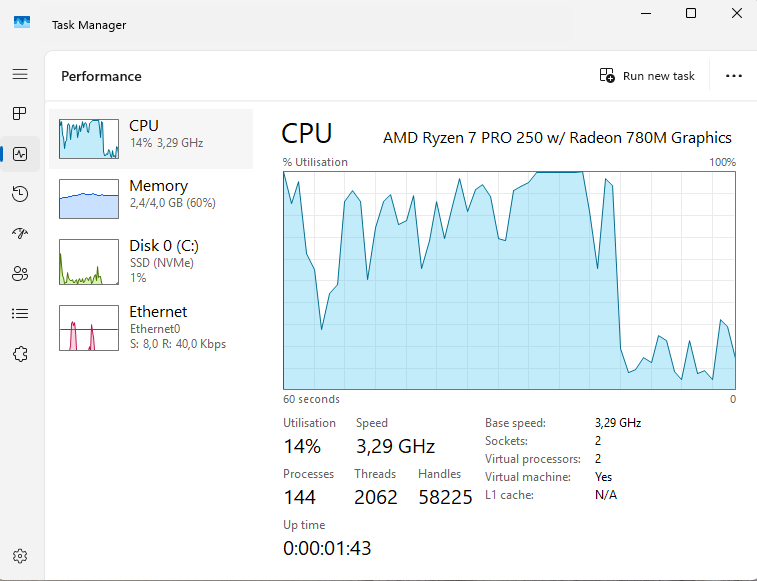
\includegraphics[width=0.99\linewidth]{taskmanager.png}%
}
\end{minipage}

